\documentclass[12pt]{article}
\usepackage{graphicx} % for inserting images
\usepackage[utf8]{inputenc} % for good practice
\usepackage{amsmath} % for equations
\title{Support Vector Regression\\using\\Deflected Subgradient Methods}
\author{FearEP\\Lord Gugger}
\begin{document}
	\begin{titlepage}
		\maketitle
		\pagenumbering{gobble}
			%\pagenumbering{arabic} per rimettere i numeri
	   \begin{center}
		\vspace{0.5cm}
	        \textit{A project presented for the\\Computational Mathematics for Learning and Data Analysis\\course}
	       \vfill	     
	       
\includegraphics[width=0.2\textwidth]{unipi.png}\\
	       University of Pisa\\
	       Artificial Intelligence\\
			A.Y. 2020/2021\\
	            
	   \end{center}
	\end{titlepage}
	
	\newpage
	\begin{abstract}
		 Project aim is developing the implementation of a model which follows an SVR-type approach including 3 different kernels. The implementation uses as optimization algorithm a dual approach with appropriate choices of the constraints to be dualized, where the Lagrangian Dual is solved by an algorithm of the class of deflected subgradient methods.
	\end{abstract}
	
	\section{Introduction}
Per affrontare questo problema di regressione ci vogliamo affidare ad un modello di apprendimento supervisionato che è il Support Vector Regression. SVR ha come obiettivo trovare una funzione tale per cui ogni record assegnatoci per il training non devii da essa più di  $\varepsilon$  (per questo ogni valore all’interno del cosiddetto $\varepsilon$-tube non viene considerato come errore nella fase di ottimizzazione, rendendo la loss del modello $\varepsilon$-insensitive). Per fare ciò abbiamo bisogno di un certo parametro C (per capire il livello di regolarizzazione che desideriamo) ed un valore $\varepsilon$ (per esprimere l’errore che accettiamo), oltre ad eventuali parametri necessari ad attuare i kernel (e.g. gamma per quanto riguarda il kernel RBF). Parte fondante del modello, oltre a ciò sopra descritto riguardo l’ $\varepsilon$-tube, è dare allo stesso tempo importanza al mantenere la funzione \textit{as flat as possible}, per evitare overfitting ed avere dunque un modello che sia un corretto tradeoff tra accuratezza e generalità.
	\begin{figure}[h]
		\centering
		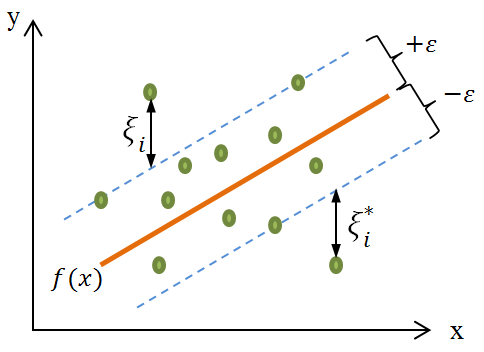
\includegraphics[width=0.5\textwidth]{svrIntro}
		\caption{a generic svr}
		\label{fig:svr_intro}
	\end{figure}

La funzione risultante dall’ottimizzazione del modello è descritta genericamente come $f(x) = w  x + b$


\end{document}